%!TEX root = ../thesis.tex
%*******************************************************************************
%****************************** Third Chapter **********************************
%*******************************************************************************
%\chapter{User preference and behaviour learning in IoT augmented spaces}
\chapter{User preference and behaviour learning in physical spaces}
\label{cha:behaviour_learning}
% **************************** Define Graphics Path **************************
\ifpdf
\graphicspath{{Chapter4/Figs/Raster/}{Chapter4/Figs/PDF/}{Chapter4/Figs/}}
\else
\graphicspath{{Chapter4/Figs/Vector/}{Chapter4/Figs/}}
\fi


%%FR In generale in questo capitolo trovo molta descrizione dello stato dell'arte. Questo dovrebbe andare nel capitolo 2. Qui dovresti iniziare a descrivere i tuoi risultati.


\section{User-space interaction}
The underlying idea that motivates the research presented in this thesis is that RSs technologies can be employed not only to support people when they interact in the virtual world,
%%FR Io enfatizzerei meglio che tu usi dati collezionati sia analizzando comportamenti online che off-line per dare supporto sia online che offline. Qui dici solo che dai supporto quando agiscono off-line.
i.e., the web, but also when they act in physical environments, i.e., a city.
This is possible due to technological advancement in the field of sensing solutions, that brought novel possibility to capture human behavioural data in real environments, i.e., recording the offline user's behaviour. Sensed user behavioural data can then be leveraged to learn user's preferences. In this thesis we mainly focus on behavioural data acquired from sensors like GPS and IoT devices, such as, beacons.

\subsection{GPS data}
The GPS sensor on the mobile device of a user provides fine-grained location data that describes the mobility behaviour of the user. This information is typically formatted as a tuple $g=(lat,lon,t,\mu)$, where $lat$ and $lon$ are the latitude and longitude of the sensed location, $t$ is a timestamp and $\mu$ is the accuracy of the measure. A GPS device can update the location at the scale of seconds and can have an error in the range of few meters. 
%So, a user that moves and is equipped with a GPS sensor creates a trajectory of gps records. 
GPS data with different configurations of location updates and accuracy are used to support users in different scenarios: short interval location updates and high accuracy measures are typically used in navigation applications where the goal is to drive a user from location A to B in real time; non-frequent and less accurate locations updates are used in LBSNs 
%%FR esplicita l'acronimo
applications in order to identify locations of interest for a user.

%GPS data by nature lacks of semantic and therefore needs to be interpreted in order to use them in an application.
GPS data are by nature  noisy and therefore need to be processed in order to be used in an application.
The field of study that aims at extracting insights from GPS traces is trajectory data mining. 
%%FR puoi mettere un riferimento a proposito?
The term ``trajectory'' indicates the fact that a GPS device generates a trajectory %$\zeta_{gps} = (g_0,\dots,g_n)$ 
$\zeta_{GPS} = (g_j: j \in \{ 0, \dots, n\})$ 
%%FR non mi piace questa notazione. Io metterei (g_0, ..., g_n)
composed of $n$ location updates. In this thesis we adopt the following trajectory data mining techniques: stay point detection; trajectory segmentation; trajectory clustering; map matching. Stay point detection techniques are employed to identify the location, 
%%FR sembra, da quello che dici, che sia invece l'indentificazione del POI dai dati di location.
within a certain radius, where a user, or any moving objects, stayed for a given time-interval. A stay point can be, e.g., a restaurant or a museum that a user has been to, and, in addition to the GPS locations in a trajectory, it carries a deeper (semantic) meaning (i.e., it describes the user's action).
%%FR ??? Action? forse si potrebbe dire "intent". Ma questo dovrebbe derivare dalla letteratura e dalle definizioni che sono usate. Non credo che questo te lo sia inventato tu.
Trajectory segmentation methods deconstruct a trajectory into sub-trajectories by time interval, spatial shape, or semantic meanings. This representation is generated before performing clustering or classification. Map matching techniques aim at projecting trajectory GPS location onto the corresponding road segment where the point was generated.
%%FR metti appropriati riferimenti

The details of the trajectory data mining techniques that we employ/designed in order to process GPS data are detailed in Chapter \ref{cha:wondervalley}.

\subsection{IoT data}
IoT technologies make possible the exploitation of sensors networks to enable new ubiquitous information services \cite{iotdef:li,li:zhao:2015}. In fact, by distributing sensors in an environment or even by integrating them into objects it is possible to respond to user actions in real time as well as collecting data about the user behaviour \cite{iot:notifications, iot-sensor-healthcare, petrelli2013integrating}.
The IoT sensors that we consider for collecting human behavioural data are those that exploit  RFID, NFC and BLE short-range wireless technology. 
%%FR metti un riferimento ad un testo dove questi concetti sono spiegati. Espandi gli acronimi.
In contrast to GPS sensors, BLE allows to capture the actions a user performs as well as their semantic. 
%%FR ??? non capisco di cosa si tratti.

Peculiar to IoT augmented scenarios is the possibility to collect user physical actions data not only outdoor, but also indoor. For instance, by augmenting a physical space like the exhibition room of a museum (indoor) or a square in the old town of a city (outdoor) with a beacon device, i.e., small BLE devices broadcasting low-energy Bluetooth messages encoded with standard transmission protocols (e.g. Eddystone or iBeacon), is possible to collect user's behavioural data.
%%FR esemplifica
The broadcasted messages can be sensed by the Bluetooth receiver of the user mobile (smartphone) and, with the aid of background processes running on the devices, can fire the generation of location-based notifications or feed information to a user model in order to support further personalization of the system generated information
\cite{iot:beaconinteracton:Ng:2017}.
In addition, IoT augmented objects enable new possibilities to collect behavioural data about the user-space interactions. Sensors enabled objects allow to detect when they are moved and manipulated. This enable the possibility to design interactive scenarios where descriptive information about objects is presented to users at the very exact time when they are inspecting them, hence, stimulating enjoyment and sharing \cite{iot:tangibleinteraction:2009}.

We represent an interaction of a user with an IoT augmented place or object as a tuple $i=(id, a, t)$. With $id$ we denote the identifier of the IoT device with which the user interacted. The action $a$ performed by the user represent the semantic of the physical action, e.g., with ``visit'' we represent the visit to a POI or with ``play'' we mean the fact that a user started a media content. With $t$ we model the time (timestamp) at which the action $a$ is performed. 
%%FR ma non metti un id dello user?
Specific of user-IoT interactions is how the (geo) location information is handled: the $id$ of the IoT device can be used to enrich the record $i$ with information about the user location by using application domain knowledge, i.e., IoT devices are deployed in fixed positions of specific areas. Alternatively, the GPS of the user mobile device can be leveraged to annotate with the location coordinates the sensed interaction. The IoT traces of a user that who interacted $n$ times with the physical environment form a list 
%$\zeta_{IoT} = (i_0, \dots, i_n)$ 
$\zeta_{IoT} = (i_j : j \in \{ 0, \dots, n\})$ 
composed of actions updates (and locations) $i$.
In order to get more information about technical aspects about the IoT infrastructure that we have designed, in order to trace and respond to user's actions in sensor enabled spaces, we refer to our study ``Tangible Tourism with the Internet of Things'' \cite{massimo:enter2018}. 

\subsection{Social Network data}
Scientists in the fields of urban computing and computational social science have investigated how user behavioural data can be derived from social networks in order to investigate mobility and socio-economic aspects in specific geographical areas \cite{urban_computing:2014, urban_computing:LBSN:2019,eating_habits:lbsn:2014}.

LBSNs 
%%FR have you explained this acronym?
offer rich information about users' interactions in the physical space. For instance, in photo sharing platforms like Instagram\footnote{\url{https://www.instagram.com/}} each photo provides additional insight (e.g., descriptive tags, likes) about a location (geo coordinates) at a given time,
%%FR Ne sei sicuro? Non mi pare che in Istagram uno metta le coordinate delle foto. Qualche volta si specifica la locazione, ma non c'e' nessun controllo che la locazione immessa sia quella corretta.
whereas in check-in platforms like Foursquare City Guide\footnote{\url{https://foursquare.com/city-guide}} a location (e.g., a POI)
%%FR per te location e POI sono la stessa cosa? Per me un POI ha una location ma una location potrebbe non corrispondere ad alcun POI.
is enriched with metadata like the POI category (bar or shop) and opinions of the users (ratings or reviews).
Even though LBSNs offer such level of information about specific places in the physical environment, user's data are generally sparse if compared to the amount of data a GPS sensor can collect. % and, moreover, due to the structure of the platform is not easy to derive sequences of visited places for a specific individual.

Besides LBSNs, more traditional social networks, such as the photo sharing platform Flickr, offer the possibility to collect user behavioural data.
%%FR Cosa distingue Instagram da Flickr?
For instance, in \cite{indoor:lbsn:2018} Flickr\footnote{\url{https://flickr.com}} photos, their related geo data and tags have been used to identify indoor activities in the cities of New York and London. In other works \cite{danub:lbsn:2019} Flickr data has been used but never considering individual photos.
%%FR Non capisco cosa vuoi dire?
In \cite{lbsn:itineraries:2010} Flickr data have been leveraged in order to automatically generate visit itineraries. 

In this thesis we leverage Flickr data because its geo-localized pictures and their metadata are more likely to be related to the place where they have been taken. Moreover, since we are interested in learning users' preferences as well as their sequential decision making to generate next-item recommendations, we leverage Flickr data to retrieve individual sequences of observations.

For a specific user of a social network or LBSN a record can be represented as a tuple $l = (lat, lon, F, t)$, where $lat$ and $lon$ are the latitude and longitude of a location, $F$ is the set of features characterizing the location, e.g., the category of a POI or aggregate feedback expressed by the community on the POI, $t$ is the time at which the user added content to the LBSN platform.
%%FR quindi potrebbe essere molto diverso da quando quella location e' stata visitata. Dovresti discutere questi problemi.
For a LBSN user is possible to build a trajectory of the $n$ locations he was physically present %$\zeta_{LBSN} = (l_0, \dots, l_n)$.
$\zeta_{LBSN} = (l_j: j \in \{ 0, \dots, n\})$.
%%FR non si capisce bene queste locations da dove vengono. In realtà quello che l'utente fa e' di aggiungere dei contenuti o di creare dei post (cioe' fa delle azioni) da cui si deriva una location.

In this thesis we collect user behavioural data from the Flickr platform. In particular, from photo albums uploaded by users on Flickr, where each photo is geo-tagged, we reconstruct the itinerary a user followed.
%%FR Tutte queste discussioni sopra sono ancora descrizione dello stato dell'arte o di cose generali che non fanno parte dei tuoi risultati.

\section{Making sense of user-space interaction data}
\label{sec:user-space_mapping}
Either we have 
%%FR Non si capisce se stai facendo un discorso generale o se veramente tu adesso descrivi qualche tecnica e risultato costruito con questi due tipi di dati.
user-space interactions (trajectories) that have been collected by means of GPS sensor on the user mobile; sensed by the users' mobile Bluetooth receiver (interaction with a Beacon); or reconstructed from the user's profile on a social network, there is the need to build a representation of each interaction with the environment that allows to infer the underlying factors (preferences) that motivates the user's (offline) behaviour.

To attain this goal we need to employ a feature representation 
%%FR di cosa?
%can capture the latent behaviour in the data in such a way that a 
that a ML 
%%FR evita se puoi di usare acronimi. Qui hai spazio.
model can exploit to learn and generalize from the data. 
%%FR un modello e' addestrato o learned a partire dai dati. Non si capisce cosa vuol dire "generalize".
We think that for any scenario in which a user performs decision making 
%%FR che decisioni? Cerca di essere piu' specifico e non rimanere sul vago.
there are two main types of information that need to be considered: context information, describing what are the conditions in which the user operated; content information describing the items subject to the user's choices.

Let assume that any data trajectory $\zeta_{GPS}$, $\zeta_{IoT}$ and $\zeta_{LBSN}$ of length $n$ can be represented by a more general trajectory $\zeta = (o_j : j \in \{ 0, \dots, n\})$ where the user-space interaction observation $o = (lat,lon,t)$ models the fact that an interaction 
%%FR non dici che tipo di interazione? Non ti interessa distinguere? In quello che abbiamo fatto abbiamo sempre parlato di POI, stato e azione. Il POI e' una particolare locazione che ha uno specifico motivo di interesse, lo stato raccoglie altre informazioni legate al fatto che l'utente era nel POI in un particolare stato, e l'azione descrive quello che l'utente voleva fare, e' l'intent. Qui faccio fatica a trovare queste idee, che poi devi usare per descrivere i modelli. Si parla solo di locazione al tempo t.
happened at the location defined by the latitude and longitude pair $(lan,lon)$ at time $t$. With $O$ we denote the set of all the user-space interactions $o$. 
%%FR A me sembrano solo locazioni visitate da qualcuno, non specificato, al tempo t.
Let $E_{ctx}$ be the set of contextual informations in an external resource, 
%%FR Non c'e' bisogno di dire "external", da un punto di vista logico non ci interessa nulla sapere da dove vengono queste informazioni, se dal telefono o da un server o dal beacon ...
%% Inoltre non si capisce che tipo di spazio e' questo E_{ctx}.
%% Siccome dopo lo usi per dire che questo ti fornisce le "features" dello spazio degli stati, o qui o dopo devi descriverlo meglio. E' uno spazio R^n, e' {0,1}^n?
e.g., the content of a weather API, and let $E_{cnt}$ be the set of content information that can be obtained from an external resource, e.g., Wikipedia.
%%FR Stesso discorso. Queste abbiamo sempre detto che sono features del POI.
That said, in order to enrich with context and content data the observations in $O$, we have to identify two mappings: 
%%FR la prima cosa che devi mappare e'una location ad un certo istante in un POI. Le features sono features del POI non della location. Dal mio punto di vista. Se per esempio sei di fronte alla chiesa dei domenicani, sei alla chiesa dei domenicani o in piazza domenicani? Magari quella \psi_{cnt} che descrivi dopo potrebbe essere pensata come il mapping da una locazione fisica ad un POI.
$\psi_{ctx}: O \rightarrow E_{ctx}$ that maps a user-space interaction $o$ to a specific context, e.g., a POI-visit is mapped with its weather conditions; the mapping $\psi_{cnt}: O \rightarrow E_{cnt}$ that maps the same user-space interaction $o$ with content information, e.g., a POI-visit is mapped to its category.

The external information resources to be employed in order to enrich the user-space interactions observations can be: (1) generated (or defined) by domain experts; (2) identified among available online resources, e.g., Wikipedia.
For instance, in order to obtain content information in the tourist domain, with the objective of learning tourists' preferences, Wikipedia and Tripadvisor can be used as external resources.
With regard to context information, it is possible to derive relevant features directly from the user-space interaction data. For instance, the crowdedness of a place can be inferred from the geo-coordinates and the time recorded in the data: by defining a bounding geographic area, all the users that interacted at a specific time in that area provides the information about the size of the crowd. For other type of context data, like the weather, online resources can be used.

Here we describe an example showing how we add, by using Wikipedia data, content and context information to trajectories of visited locations in a city.
Content data falling within a geographic (bounding-box) area, defined by the minimum and maximum values of the $(lat,lon)$ pairs in the data, is retrieved from the external information source. %For instance, for a user trajectory of visited locations derived from a LBSNs the external source of information can be Wikipedia. 
%All the geo-localized Wikipedia pages that falls in the bounding box derived from the users' trajectories, minimum and maximum values of the $(lat,lon)$ pairs in the data, can be downloaded and then processed to identify a set of features, e.g., the place name and its type (bar or shop), to represent the location. 
Then, the retrieved content is processed to identify a set of features, e.g., the place name and its type (bar or shop), to represent the location. 
Afterwards, each location in a trajectory can be enriched with the identified content. In this way a pair of geographical coordinates becomes a recognizable POI and the trajectory becomes the itinerary of POI-interactions the user made in the physical space. From such, richness of information in the data user behaviour information can be learnt.

\section{Learning a user preference model}
\label{sec:learning_user_preferences}
In this section we detail how we learn user's preferences and behaviour from observed user-space interaction trajectories.
In particular, we present how we model the problem of the trajectory generation task, which is closely tight to the problem of sequential decision making. Afterwards, we detail how we  learn user' preferences as well as her action-selection policy. 

\subsection{Problem modelling}
%\textbf{Markov Decision Process Model.} 
We model the user-space interaction trajectory generation task
%%FR Non sono convinto che questo risolve in "generation task". Devi aver gia' generato le trajectories per costruire il tuo MDP. MDP e' il modello formale in cui sistematizzi il problema decisionale dell'utente, non le traiettorie, che sono delle sequenze di azioni.
as a finite Markov Decision Process (MDP). A MDP is defined by a tuple $(S,A,T,r,\gamma)$. With $S$ we denote a finite set of states and in our scenario a state represents the interaction of a user with the physical space (e.g., visiting a POI) in a specific context (e.g., weather, temperature and day). For instance, a tourist that visits the old town of Florence can be at the Battistero (POI) in a cloudy, cold morning (context). $A$ is a finite set of actions, which in a tourism scenario can represent the decision to move to a POI. With $T$ we indicate a finite set of probabilities $T(s'| s, a)$, to make a transition from state $s$ to $s'$ when action $a$ is performed. For example, a user that visits Battistero in Florence during a cloudy morning (state $s_1$) and wants to visit the Uffizi Gallery (action $a_{1}$) in the afternoon can arrive to the desired POI with either a cloudy sky (state $s_2$) or a clear sky (state $s_3$) with transition probabilities $T(s_2,a_{1}|s_1)=0.5$ and $T(s_3,a_{1}|s1)=0.5$.
The function $r: S \rightarrow \mathbb{R}$ models the reward a user obtains from visiting a state. This function is supposed to be {\it unknown} and must be learnt, i.e., we take the restrictive assumption that we do not know the utility the user receives from her interaction with the environment (the user is not supposed to reveal it). But, we assume that if the user performed an action and not another one, then she believes that the first action gives her a larger utility/reward than the second. Finally, $\gamma \in [0,1]$ is used to discount future rewards with respect to immediate ones. 
%
We denote with $\zeta_u$ a user $u$ trajectory,
%%FR Lo avevi fatto anche prima ma le traiettorie erano prima sequenze di locazioni. Devi evitare questa confusione. Hai troppi di tipi di traiettorie. Magari puoi distingure tra traiettorie di locazioni e traiettorie di stati. Le prime sono le osservazioni fisiche e le seconde sono arricchite da altre informazioni (contesto, intent dell'utente, features del POI, ecc).
which is a temporally ordered list of state-action pairs (user-space interactions). 
%%FR In un MDP si parla di sequenze di stati non di stati-azione. Hai davvero bisogno di parlare di stato-azione. Noi abbiamo sempre inteso che lo stato descrive anche l'azione, ovvero se un utente e' in un POI vuol dire che voleva visitare questo POI. Non abbiamo casi in cui un utente voleva visitare il POI a e si trova invece al POI b. Puoi lasciare stato-azione ma se non serve crea solo confusione.
For instance, $\zeta_{u_1} = ((s_{10},a_{3}), (s_5,a_8), (s_{15}, a_e))$ represents a user $u_1$ trajectory starting from state $s_{10}$, moving to $s_5$ by performing action $a_3$ 
and ending to $s_{15}$ by acting according to $a_8$. The last action $a_e$ is a dummy action that indicates the end of the trajectory. With $Z$ we represent the set of all the observed users' trajectories. 
%
Given a MDP, our goal is to find a policy $\pi^* : S \rightarrow A$ that maximises the cumulative reward that the decision maker obtains by acting according to $\pi^*$ (optimal policy). 
The value of taking a specific action $a$ in state $s$ under the policy $\pi$, is computed as :

$$Q_{\pi}(s,a)=\mathbf{E}^{s,a,\pi}[\sum_{k=0}^{\infty} \gamma^k r(s_k)]$$

i.e., it is the expected discounted cumulative reward obtained from $a$ in state $s$ and then following the policy $\pi$.

%\begin{equation}
%\label{eq:bellman} 
%Q_{\pi}(s,a) = \sum_{s'}T(s'|s,a)r(s')+\gamma \max_{a'}{Q_{\pi}(s',a')}
%\end{equation}

The optimal policy $\pi^*$ dictates to a user in state $s$ to perform the action that maximizes $Q_{\pi^*}$. So, in order to compute $Q_{\pi^*}$ we rewrite the previous formula as:

$$Q_{\pi^*}(s,a) = \sum_{s'}T(s'|s,a)\left[r(s)+\gamma \max_{a'}{Q_{\pi}(s',a')}\right]$$

%%FR sei sicuro di questa formula? Il Q tra parentesi non e' relativo a pi^*? Non e' la formula di Bellman?

The problem of computing the optimal policy for a MDP is solved by Reinforcement Learning algorithms \cite{sutton:1998}.

As we mentioned earlier, in a information systems and specifically in RSs applications the reward obtained by a user when she is in a specific state (i.e., the $r$ function) is usually unknown because users scarcely provide feedback (e.g., ratings or reviews about the consumed items). Therefore, we are interested in determining the reward function $r$ from the bare observations of the decision maker transitions from state to state; this problem is solved by Inverse Reinforcement Learning (IRL). 


\subsection{IRL}
%%FR Secondo me queste cose generali su MDP e IRL andrebbero nello stato dell'arte e qui dovresti spiegare come lo hai applicato al nostro dominio. Ora magari e' troppo complesso separare. Ma dovresti cercare piano piano di sposatre nello stato dell'arte le cose generali in modo che qui la discussione e' davvero specifica.
IRL algorithms take as input a model of the environment, the MDP, and the observed behaviour of a user (or any autonomous agent) in the form of demonstrations, in our case the trajectories in $Z$,
%%FR Le traiettorie di stato o di stato-azione?
and return the inferred user's reward function. In IRL the underlying assumption is that a user is a rational decision maker who seeks to optimize the reward associated to her actions. Due to this, the agent is typically referred as ``expert''.

Generally the state space $S$ is represented by a state feature function $\Phi:S \rightarrow \mathbb{R}$ that assigns to each feature a real value.
%%FR ??? Questa sara' una funzione in R^n non in R perche' uno stato e' descritto da molte features non una.
We model each state by using the features identified with the mappings $\Psi_{cnt}$ and $\Psi_{ctx}$ (Section \ref{sec:user-space_mapping}).
%%FR Come dicevo prima, devi spiegare meglio che tipo di spazio e' questo e magari fare un esempio concreto che aiuta a capire.
%For instance in the tourism domain a reasonable set of state features that can be used to infer the reward a tourist obtains from observations of POI-visit, can be: the type of a POI; opening hours; the weather; the day of the week; amount of visitors; the price range. 


In order to infer the user's reward from her observations there is the need to identify a solution, i.e., a reward function, that makes the observed behaviour optimal. 
IRL algorithms can reconstruct the reward function $r$ and the optimal action-selection policy $\pi^*$ of a user $u$ from the set of her observed trajectories. We assume (as in \cite{ng:2000}) that $r$ is a linear function, $r(s) = \theta^T\phi(s)$, of the state $s$ feature vector $\phi(s)$ 
%%FR perche' ora la funzione che produce le features e' phi minuscolo e prima era Phi maiuscolo?
and the user utility vector $\theta$, which models the unknown user preference for the state features. IRL algorithms derive the user's action-selection policy from the learned reward function $r$ by assuming that users act in order to maximise the reward.

Researchers in the field of IRL showed that the reward estimation problem is ill-posed because there is an infinite number of solutions, e.g., a reward function $r=c$, where $c$ is a constant, is an example of such problem.
%%FR Non si capisce cosa vuoi dire. Che se la reale funzione di reward e' una costante allora qualunque funzione costante e' anche una soluzione? Spiega meglio.
Therefore, the challenge in IRL is to seek for a solution that is optimal, the best among the set of all the solutions. 
%%FR Cosa vuol dire "the best"? Il problema che hai descritto sopra e' che non esiste UNA best, ma ne esistono MOLTE e che non si puo' dire qual'e' quella che l'utente sta realmente usando, assumendo che lui ne usa una sola.
The main difference among the IRL algorithms proposed in the literature is in how the solution is computed, i.e., they differ in the optimality criterion.
%%FR Quindi? Ne trovano una tra le tante soluzioni ottime? Vuoi dire questo? Sembra qusi che dici che hanno diversi criteri di ottimalita'. Questo e' fuorviante. Trovano diverse funzioni di reward che pure determinano la stessa policy ottima.

To resolve the issue of identifying an optimal solution in \cite{ng:2000,irl:optimal_solution:2006} has been proposed to add a margin in order to maximize the difference between the reward derived from the optimal policies an the reward that is derived from the alternative policies.
%
In \cite{bayesianIRL} the authors tackle the problem of computing the reward from a Bayesian perspective. The proposed model, called Bayesian IRL, leverages the users' observations in order to infer the optimal reward. At first, it uses the observations as evidence to update the prior knowledge on the set of possible reward functions (solutions), which are assumed to be independently identically distributed. Then, Bayesian IRL estimates the reward using the posterior knowledge.
%
The authors of Maximum-Entropy IRL \cite{maxentirl} propose to seek for a reward function by matching state features in the observation data. Maximum-entropy is used to identify action (i.e., user-space interactions in our case) probabilities that lead to a reward that supports the observed data.
%%FR Queste sono cose generali che andrebbero messe nello stato dell'arte su RL e IRL. Qui interrompono la discussione specifica alla tua applicazione.

\subsection{Maximum Log-Likelihood IRL}
In this thesis, in order to learn both the user's reward and her action-selection policy, we use a specific IRL algorithm called Maximum Log-likelihood (MLIRL) \cite{vro:litt:2011}. 
MLIRL combines many positive features of other IRL models \cite{bayesianIRL,maxentirl,policymatchingirl}: it assumes a prior knowledge of the user preference vector to estimate an initial reward function that is then adjusted by looking for a maximum likelihood model that can justify observed trajectories; it optimizes user behaviour via a gradient method and assumes that each user randomizes the action selection process at the level of individual choices, i.e., by sampling choices (actions) from a Boltzmann distribution. 

%In MLIRL it is assumed that experts randomize individual action choices. Choice actions are sought by the maximum likelihood solution via the gradient ascent approach. 
The algorithm exploits the fact that a guessed $\theta$ induces a probability distribution over action choices and hence determine a likelihood for the observations in $Z$. Expected values (discounted) are computed via the following formula:
% Add Bellman equation somewhere before

%\begin{equation}
$$Q_\theta(s,a) = \theta^T\phi(s)+\gamma\sum_{s'}T(s,a,s')\frac{\sum_a Q_\pi(s,a)e^{\beta Q_\pi(s,a)}}{\sum_{a'}e^{\beta Q_\pi(s,a')} }$$
%\end{equation}

MLIRL looks for $\theta = \arg\max_\theta L(Z|\theta)$ which is the maximum likelihood solution that is found via gradient ascent optimisation. 
The log likelihood of the observed trajectories $Z$ is defined as:

%\begin{equation}
$$L(Z|\theta) = \prod_{i=0}^{|Z|} \prod_{s,a \in \zeta_i} \pi_\theta(s,a)$$
%\end{equation}

The term $\pi_\theta(s,a)$ in the previous equation represents the Boltzmann action-selection policy, which is defined as:

$$\pi_\theta(s,a) = \frac{\sum_a Q_\pi(s,a)e^{\beta Q_\pi(s,a)}}{\sum_{a'}e^{\beta Q_\pi(s,a')}}$$

The computation of $\theta$ via gradient ascent is performed for a fixed number of steps $M$. At each step the $\pi_\theta(s,a)$ is computed by solving via value iteration the MDP, using the estimated reward $r(s) = \theta^T \phi(s)$.

MLIRL is known to converge to a solution in finite-horizon settings and is also known to produce a well-defined answer. The problem of the existence of multiple reward functions for which an observed trajectory is optimal in a given MDP, is solved by assigning high probabilities to observed behaviour and low probability to the unobserved. The general steps of the code are listed in algorithm \ref{code:mlirl}.

\begin{algorithm}
	\caption{Maximum Likelihood Inverse Reinforcement Learning}
	\label{code:mlirl}
	\begin{algorithmic}
		\State \textbf{Input:} S, A, T, $\gamma$, $\phi$, $Z=\lbrace \zeta_1, \dots,  \zeta_N \rbrace$, M, $\lambda_t$ step size.
		
		\State $\theta \leftarrow$ Initialize with random values;
		\For{t=1 to M} 
		\State Compute $Q_{\theta_t}$,$\pi_{\theta_t}$
		\State $L = \sum_{i} \Pr{(\zeta_i)} \sum_{(s,a) \in \zeta_i} \log{\pi_{\theta_t}(s,a)}$
		\State $\theta \leftarrow \theta + \lambda_t\nabla{L}$
		\EndFor
		\State \textbf{Output:}  $\theta$
	\end{algorithmic}
\end{algorithm}

\section{Learning from scarce individual's behavioural data}
\label{sec:clustering like behaving users}
%Finally, we show how the problem of learning an individual behaviour model from scarce user behavioural data, a common problem in information systems, can be alleviated by clustering trajectories of like-minded users and then learning a (one per cluster) generalized behavioural model.

As we have shown in the previous section by harnessing behavioural data of an individual, i.e., user-space interaction trajectories, we can learn with IRL the user behavioural model in terms of the user's preferences $\theta$, her reward $r$ and the associated action selection policy $\pi^*$. 
%%FR Non e' che questo lo hai mostrato bene. Hai descritto MDP, hai detto che con IRL puoi stimare la reward, hai forse detto che con la reward function uno puo' calcolare anche la policy ottima. Secondo me tutto questo e' poco chiaro. Non hai mai mostrato esempi e hai mescolato cose generali a cose specifiche. Secondo me le cose generali su RL e su IRL andrebbero nello stato dell'arte e magari con degli esempi classici per far capire cosa succede in quei casi. Qui dovresti solo focalizzarti sul tuo caso specifico e far capire come queste tecniche generali sono state utilizzate da te.

Generally, in information systems 
%%FR cosa sono questi "information systems"? Cerca di essere piu' specifico. Tu ti sei occupato di una particolare applicazione nell'ambito del turismo. Parla di quello se no uno come fa a capire a cosa ti riferisci?
the amount of individual user behavioural data is not large for the majority of the system users. The lack of user's data becomes more evident when it comes to user-space interaction data, for which the available public datasets are not many (and sparse as well) and the only rich datasets are those owned by service providers like Google, Foursquare, and Uber.
%%FR Io direi le cose in modo diverso, altrimenti sembra che tu abbia sviluppato una tecnica solo perche' non hai accesso ai dati. Devi valorizzare l'idea del clustering piuttosto che descriverla come un ripiego.
We think that from a RSs perspective, which is the focus of this thesis, using only target user (specific) behavioural data
%, even a rich set of individual data, 
for recommendations generation for him is of scarce utility for the user: 
%%FR in realtà nessun RS, a parte quelli content-based, usa solo i dati del target user per fare raccomandazioni a lui. In CF si usano i dati di una popolazione di utenti.
the suggested items (e.g., POI-visits) will (probably) be those that the user would choose without the help of the RS. 
%%FR E' il tipico problema dei CB RSs.
Moreover, individual behavioural data may present a sub-optimal behaviour. e.g., a user that visits for the first time a city may simply visit the few, more accessible, places that are closer to the city main attractions. Learning a behavioural model from such observations would lead to a biased model. We think that by learning, instead, a behavioural model from observations of more visitors 
%%FR ma devi dire cosa vuol dire "more" in questo contesto.
in the city, the resulting learnt behaviour will minimize the impact of sub-optimal behaviours that could influence some of the observed trajectories.

In order to alleviate the problems of learning from scarce user's data and minimizing the impact of suboptimal behaviours present in the data, we propose to group the user-space interaction trajectories in clusters and then to learn a ``general'' user behavioural model common for all the users/trajectories in a cluster.

By applying MLIRL on each cluster of trajectories we therefore learn cluster specific reward functions and behaviour models of the users in each cluster. This is the optimal policy that dictates for each state the best action, e.g., the next POI visit, the users in a cluster should take in order to maximise their reward.

%\subsection{Alleviating the problem of scarce individual users' interaction data via clustering}
\subsection{Clustering like-behaving users}
Clustering the trajectories is implemented 
%%FR Dove???? Non si capisce chi lo fa questo.
with Non Negative Matrix Factorization (NMF)
\cite{nmf:majorcontribution:1999}, which is a specific class of Matrix Factorization models. Matrix Factorization has the objective of reducing an input matrix into its constituent parts in order to ease the computation of more complex matrix operations or inspect the input data. 

Applications of NMF can be found in many field of science, e.g., in astronomy, NMF is used to process space observation data in order to identify planets that cannot be directly observed due to the high amount of light that stars close to the planet emits \cite{nmf_astronomy:2018}; in biology, NMF has been used to cluster gene expression \cite{nmf_biology:2012}. Of our interest is the application of NMF in text mining where NMF allows to group documents to a common semantic structure that can explain the resulting clusters.
%%FR Spiega quali sono i documenti che usiamo noi.

NMF requires as input a positive real valued matrix, therefore documents needs to be represented by using an appropriate statistic, i.e., term frequency–inverse document frequency (tf-id). Given a set of documents, i.e., a text corpora, the tf-idf statistic represent numerically how important is a term in a document. Let $d \in C$ be a document belonging to the corpus $C$ and let be $t \in d$ a term of the document. The tf-idf is computed by means of the following formula:
%%FR di nuovo roba generale che andrebbe nello stato dell'arte.

$$tfidf_{d,C}(t) = tf_d(t) \cdot idf_C(t)$$

The term $tf_d(t)$ is the term frequency of the term $t$ for the document $d$; we compute it as 
%$tf(t,d) = \frac{\sum_{j\in d}\textbf{1}_{j,d}}{|d|}$. The indicator function $\textbf{1}_{t,d}$ has value 1 if the term $t$ is present in document $d$, otherwise 0. 
$tf_d(t) = \frac{count_{d}(t)}{|d|}$. The numerator $count_d(t)$ is the number of terms in $d$ that are equal to $t$. 
%%FR e il denominatore?
%% Ma non usi anche qui il logaritmo della frequenza? 

The second term in the formula is the inverse document frequency $idf_C(t)$ and express how much a word is important, i.e., a word is rare or common in the corpora $C$. We compute it as:
%%FR non e' che lo calcoliamo noi cosi', questa e' una definizione generale.

$$idf_C(t)=log \frac{|C|}{|d\in C: t\in d|}$$ 


In order to use NMF to identify like-behaving/minded users from their user-space interactions trajectories we need to build a document-like representation of the trajectories. To generate such representation we harness (for each trajectory $\zeta$) the mappings $\Psi_{cnt}$ and $\Psi_{ctx}$ that we defined in Section \ref{sec:user-space_mapping}. We recall that these mappings identify descriptive features for each user-space interaction in the data. 
%%FR qui intendi per features delle keywords, ovvero il valore delle features. Penso. E' difficile dire perche' prima non descrivi bene le funzioni che mappano una locazione in un contesto o in un contenuto.
For instance, if the user visited a museum the descriptive features associated to the interactions can be: content information describing the visited place, e.g., the type of museum (science), the exhibition style (interactive); context information, e.g., the part of the day (afternoon), the weather (rainy) and the crowdedness of the place.
By representing each observed user-space interaction with its associated features (terms), we generate a document that describes the observed interaction of the user with the environment. When this operation is performed by using all the trajectories in the database we obtain the corpora that describes the interactions of all the users. 

With $D$ we denote the tf-idf matrix representation of the obtained corpora.
%We denote with $D$ the \textit{tf-idf} matrix representation of the obtained corpus. 
Columns in $D$ represents specific terms and rows corresponds to trajectories. 
The matrix $D$ has size $|Z| \times F$, where $F$ is the number of unique terms in the corpora. NMF approximates the matrix $D$ with the product of two non-negative matrices $W$ (of size $F \times K$) and $H$  (of size $|Z| \times K$).
%%FR Ma allora sara' HW^T. Scrivi la formula di approssimazione se non non si capisce cosa dici.
The matrix $H$ identifies which topics (columns) are more relevant for each user trajectory (row), and using it we assigned a trajectory to the topics that in its corresponding row have values larger than a threshold $\tau$ as similarly done in \cite{nmf:multilabelannotation:2017}. Hence, each topic defines a cluster of trajectories.
Moreover, a topic, can be described by its top terms, i.e., those with the largest values in the corresponding row in $W$.

In order to identify the correct number of topics (clusters) we conduct  a stability analysis, as suggested in \cite{topicmodeeling:greene2014}.
The procedure seeks for the best number of topics $k$ from a pre-defined space. At first, a reference $k$-topic model $M^{ref}$ is generated by using the whole corpora.  The reference model $M^{ref}$ comprises the lists of $m$ top terms of each topic. Then, a fixed number of documents subsets are sampled (without replacement) from the corpora. 
%%FR Ma quando spieghi quello che hai fatto tu???? Questa sembra ancora roba generale.
%% Qui devi descrivere per filo e per segno quello che hai fatto, non solo le tecniche generali.
%The reference model $M_{ref}$ comprises the lists of $m$ top terms of each topic and is used to assess the stability of the topics generated by corpora subsets for different $k$ values.
For each documents subset $G_i$ we generate the $k$-topic models $M$ and compute the agreement between the reference model $M^{ref}$ and $M$. With $\mathcal{M}$ we denote the set of $k$-topic models built from $G_i$. The computation of the agreement between two $k$-topic models is performed by: (1) building a square matrix $J$ containing the average jaccard values of the $k$ topics in $M^{ref}$ (rows) and the $k$ topics in $M$ (columns); (2) computing the agreement score $agree(M^{ref},M)$.

In particular, the average jaccard score for the $k$-th topic, with $m$ top words, in $M^{ref}$ and $M$ is computed using the formula:

$$\overline{jacc}(M^{ref}_{k}, M_{k}) = \frac{1}{m} \sum_{l=0}^{m} \frac{|M^{ref}_{k,l} \cap M_{k,l}|}{|M^{ref}_{k,l} \cup M_{k,l}|}$$

The agreement score for the 
%$$agree(M^{ref},M)=\frac{1}{k} \sum_{i=1}^{k} \overline{jacc}(M^{ref}_{k}, best_{\overline{jacc}}(M_{ref,k},M_{i,k})) $$

$$agree(M^{ref},M)=\frac{1}{k} \sum_{i=1}^{k} \max{J_k}$$

Finally the stability is computed as:

$$stability(k) = \frac{1}{|G|} \sum_{i=1}^{|G|}agree(M^{ref},\mathcal{M}^i)$$

The best number of topics/clusters $k$ is the one with highest stability score (mean agreement).
%%FR ma non si capisce come cerchi nello spazio di tutti i possibili k. Hai detto che parti da un k e non dici che valore ha, e poi non dici quali altri valori di k provi.

\section{Case study: Learning user preferences and behaviour in open spaces}
%%FR Io non lo presenterei come "case study" se no sembra solo che tu hai fatto un case study con tecniche ben note. Se presenti le cose in questo modo togli valore al tuo lavoro.

%In ``L'' \cite{} we show an example of learning user's behaviour in an indoor IoT augmented space.
In this case study we present how user-space interaction data can be leveraged to learn tourists' behaviour in the scenario of visiting a cultural heritage centre. %User's visit actions trajectories are acquired from the Flickr photo sharing platform and additional content and visit context information have been retrieved from Wikipedia and a weather API.

\subsection{Available data}
The dataset we employ consists of 1663 users' POI-vist trajectories in the city of Florence (Italy) that have been reconstructed by employing data harvested from the Flickr photo sharing platform.
%%FR ma non l'hai fatto tu. Devi dire chi ha fatto cosa in maniera chiara.
%Tourists' offline behavioural data have been retrieved from the Flickr\footnote{https://flickr.com} photo sharing platform.
The POI-visit trajectories are built by following the general example presented in Section \ref{sec:user-space_mapping}.
In particular, images in a Flickr photo album are tagged with information about the geographical coordinates and the shooting time, from these information a trajectory 
%%FR prima hai dato diverse definizioni di traiettoria. Cos'e' ora una traiettoria? Usa le definizioni che hai dato.
is constructed as follows: (1) geographical coordinates are used to represent the picture as a recognizable POI by fetching relevant content data from an external source; (2) the shooting time is used to order the identified POIs in such a way that we obtain a temporally ordered list of user's visited POI, i.e., the user itinerary. 
%%FR Ma non puoi ora descrivere ora con precisione le varie funzioni che hai descritto sopra e che fanno parte del tuo modello generale?
So, photo albums which elements fall within the geographical boundaries of the city of Florence\footnote{\url{https://www.openstreetmap.org/relation/42602\#map=12/43.7716/11.3291}} have been downloaded and sorted.
%%FR lo hai fatto tu?
Each photo is then matched with the Wikipedia pages whose geographical coordinates fall within the Florence area. The matching procedure is done by defining a circular area, with fixed radius ($r=100$ meters), centred in the photo coordinates and then by seeking  for the closest Wikipedia content geo-localized in that area.
In this case study we use as starting point the POI-visits trajectories dataset presented in \cite{flikr_tourism_RS:muntean:2015}.
%%FR quindi il match lo hanno fatto loro? Devi essere piu' preciso nel dire quello che hanno fatto loro e quello che hai fatto tu.
We manually added to each POI-visit data content information about the POI itself by using expert knowledge extracted from the POI Wikipedia page. Since all the identified POIs are cultural attractions we decided to identify the following set of features to represent them: 
%%FR questo lo devi descrivere bene e motivare perche' ha un impatto notevole sul modello comportamentale.
the POI category (e.g., monument), the historical period (i.e., century) and one historical person related to the POI. In the 532 POIs appearing in the trajectories we identified 13 different POI categories, 18 historical periods and 106 historical persons. 
With regard to the visit context of a POI-visits we leveraged the timestamp (the date) and the geographical coordinates of each POI-visit to query a weather service\footnote{\url{https://darksky.net}} to collect an hourly weather summary (e.g., cloudy), temperature (e.g., cold) and daytime (e.g., evening). 
%%FR Anche questo deve essere motivato meglio perche' ha un impatto sul modello comportamentale che poi apprendi.

The trajectories/users ratio is 1.43 and the average trajectory length is 11.7 POI-visit. 
%%FR e cosa vuol dire questo? Spiega, commenta.

\subsection{Identification and inspection of like-behaving users}
In order group like-behaving users in the dataset we apply the approach described in Section \ref{sec:clustering like behaving users}. So, we generated a text corpora by building a document-like representation for each trajectory. The terms in the corpora are the content and context features associated to the POI-visits. Then, we applied NMF and we identified 5 different trajectory clusters.
In Table \ref{tab:Topics} we show the top-10 terms per cluster and the number of associated trajectories. Clusters are named with the first 5 English alphabet letters.

\begin{table}[h]
	\centering
	
	\caption{Top 10 terms in the five topics extracted from the trajectory data set and number of trajectories assigned to each topic (cluster).}
	
	\label{tab:Topics}
	\begin{tabular}{ |l|l|l|l|l|l| }
		\hline
		\textbf{\#Term} & \textbf{Cluster A} & \textbf{Cluster B}  & \textbf{Cluster C}& \textbf{Cluster D} & \textbf{Cluster E}  \\ \hline
		1  & morning &hot &cloudy &warm &freezing   \\ \hline
		2  & cold &afternoon &cold &cloudy &cloudy   \\ \hline
		3  & square &century 16 &church &century 14 &afternoon   \\ \hline
		4  & palace &palace &square &church &century 14   \\ \hline
		5  & century 15 &church &century 13 &square &palace   \\ \hline
		6  & century 13 &square &palace &building &building   \\ \hline
		7  & church &century 19 &rain &palace &century 13   \\ \hline
		8  & night &century 13 &museum &ponte &church   \\ \hline
		9  & dante &museo &brunelleschi &century 13 &foggini   \\ \hline
		10 & century 10 &brunelleschi &tadda &century 19 &century 19   \\ \hline
		\hline
		\textbf{\#Traj.} & 368 & 339 & 341 & 297 & 153 \\ \hline
		
	\end{tabular}
\end{table}

In the following, we exemplify the results of the clustering step by comparing two cluster examples (i.e., C and E); they have some similar features but a different number of trajectories. Figure \ref{fig:cluster_map} depicts the clusters' trajectories and 15 most popular POIs.

\begin{figure}
	\centering
	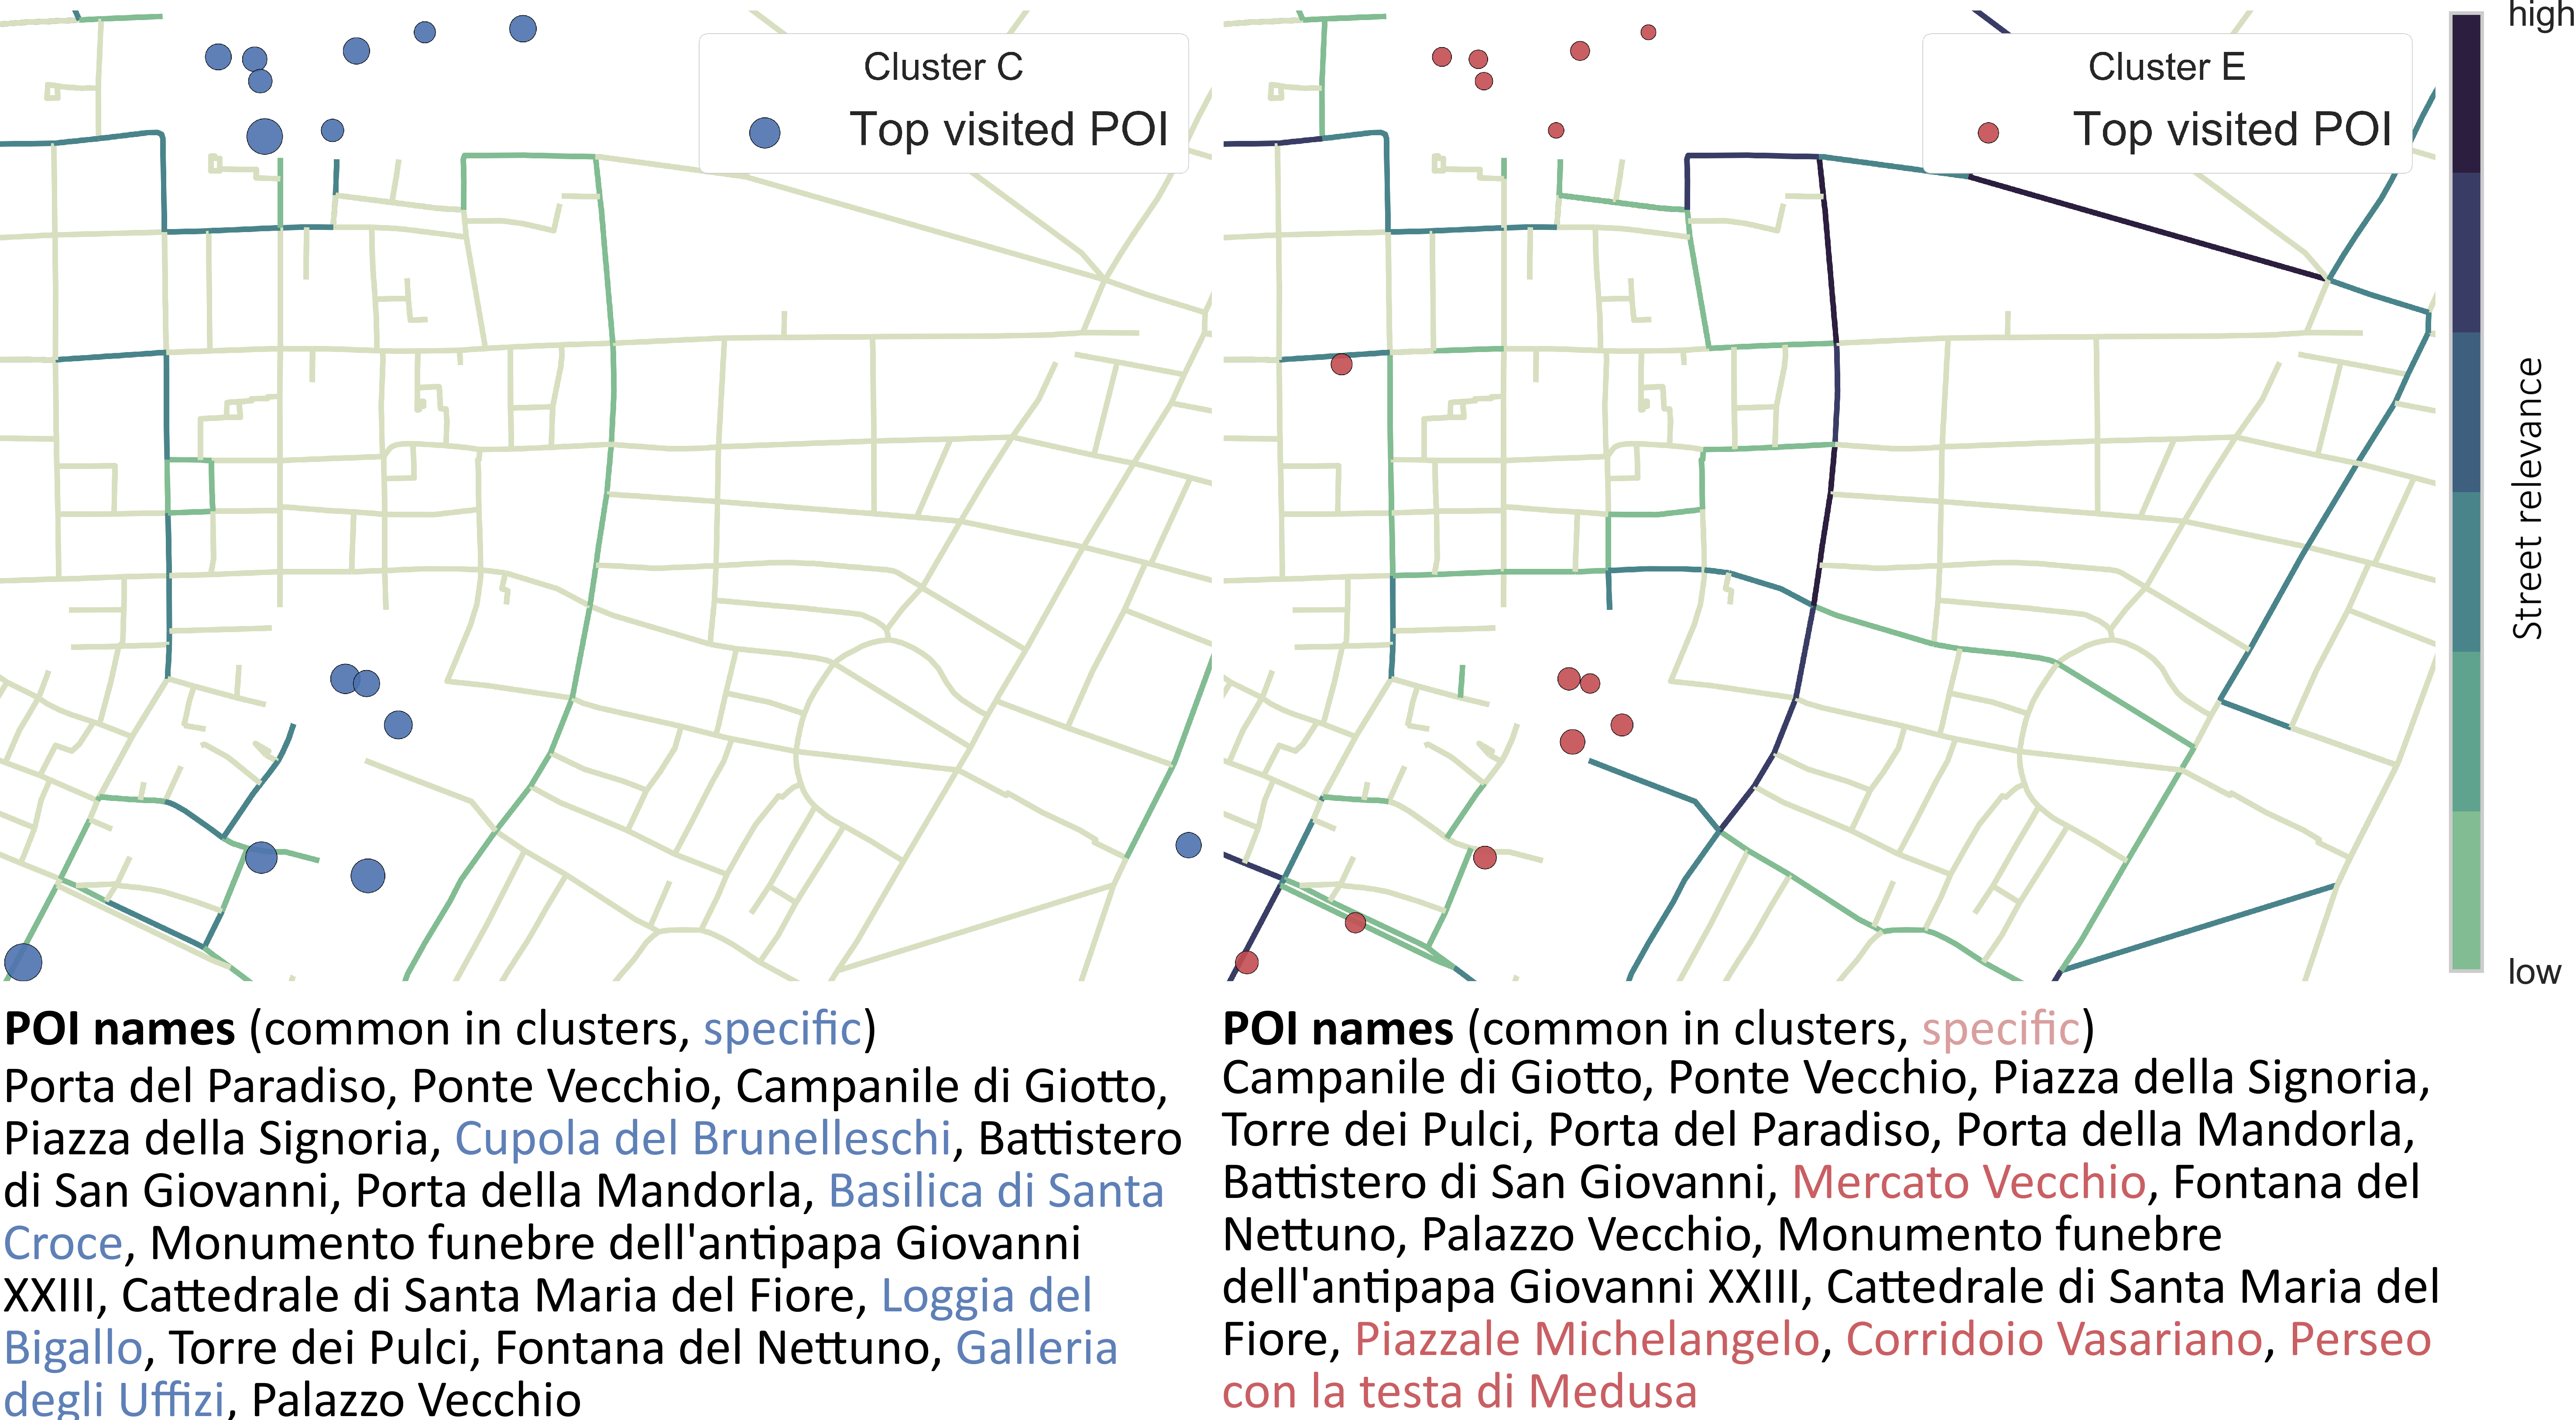
\includegraphics[width=\linewidth]{cluster_comparison_poinames}
	\caption{Top-15 visited POIs and street relevance (heatmap) for two clusters}
	\label{fig:cluster_map}
\end{figure}

The POIs are depicted as circles with diameter proportional to the normalised POI popularity:  the more popular the POI is in the cluster the larger the circle is. There is a large number of POIs present in both clusters, but they differ in terms of normalised visit frequency. In fact, in the cluster represented on the right (cluster E), POI circles are smaller because of a more uniform distribution of the visits among all the POIs in the cluster (i.e., not only the top-15 shown in the figure). 
An aspect that we see of particular interest is related to how users interacts with the surrounding environments. To show that, in Figure \ref{fig:cluster_map} we show how important are the streets of Florence for the clustered users/trajectories.
The importance of the various streets in the clustered trajectories is determined by identifying the most representative trajectories in the clusters. These are the trajectories whose \textit{tf-idf} vector representation is closer, in cosine similarity, to the cluster centroid, which is the average vector of all the \textit{tf-idf} vector trajectory representations. The street importance is represented as shades of the colour bar on the right part of the figure; it has higher values (darker colour) in proximity to popular POIs and on the main streets connecting them. 

At the bottom of Figure \ref{fig:cluster_map} the most popular POIs in the two clusters are listed. POI in black typeface are common to the two clusters, whereas coloured POIs are cluster specific. 11 POIs are common to these two clusters and 9 of them are common to all the clusters. They actually belong to the top-15 attractions according to popular travel portals\footnote{
	\url{www.planetware.com/tourist-attractions-/florence-i-to-f.html} \\  
	\url{www.touropia.com/tourist-attractions-in-florence/} \\ \url{theculturetrip.com/europe/italy/articles/20-must-visit-attractions-in-florence-italy/}
}.

We show additional clusters differences in Figure \ref{fig:cluster_poi}, where POI features per cluster are compared.
This figure shows the probability of various features (POI category, historic period and related person features) in the five considered clusters.

\begin{figure}
	\centering
	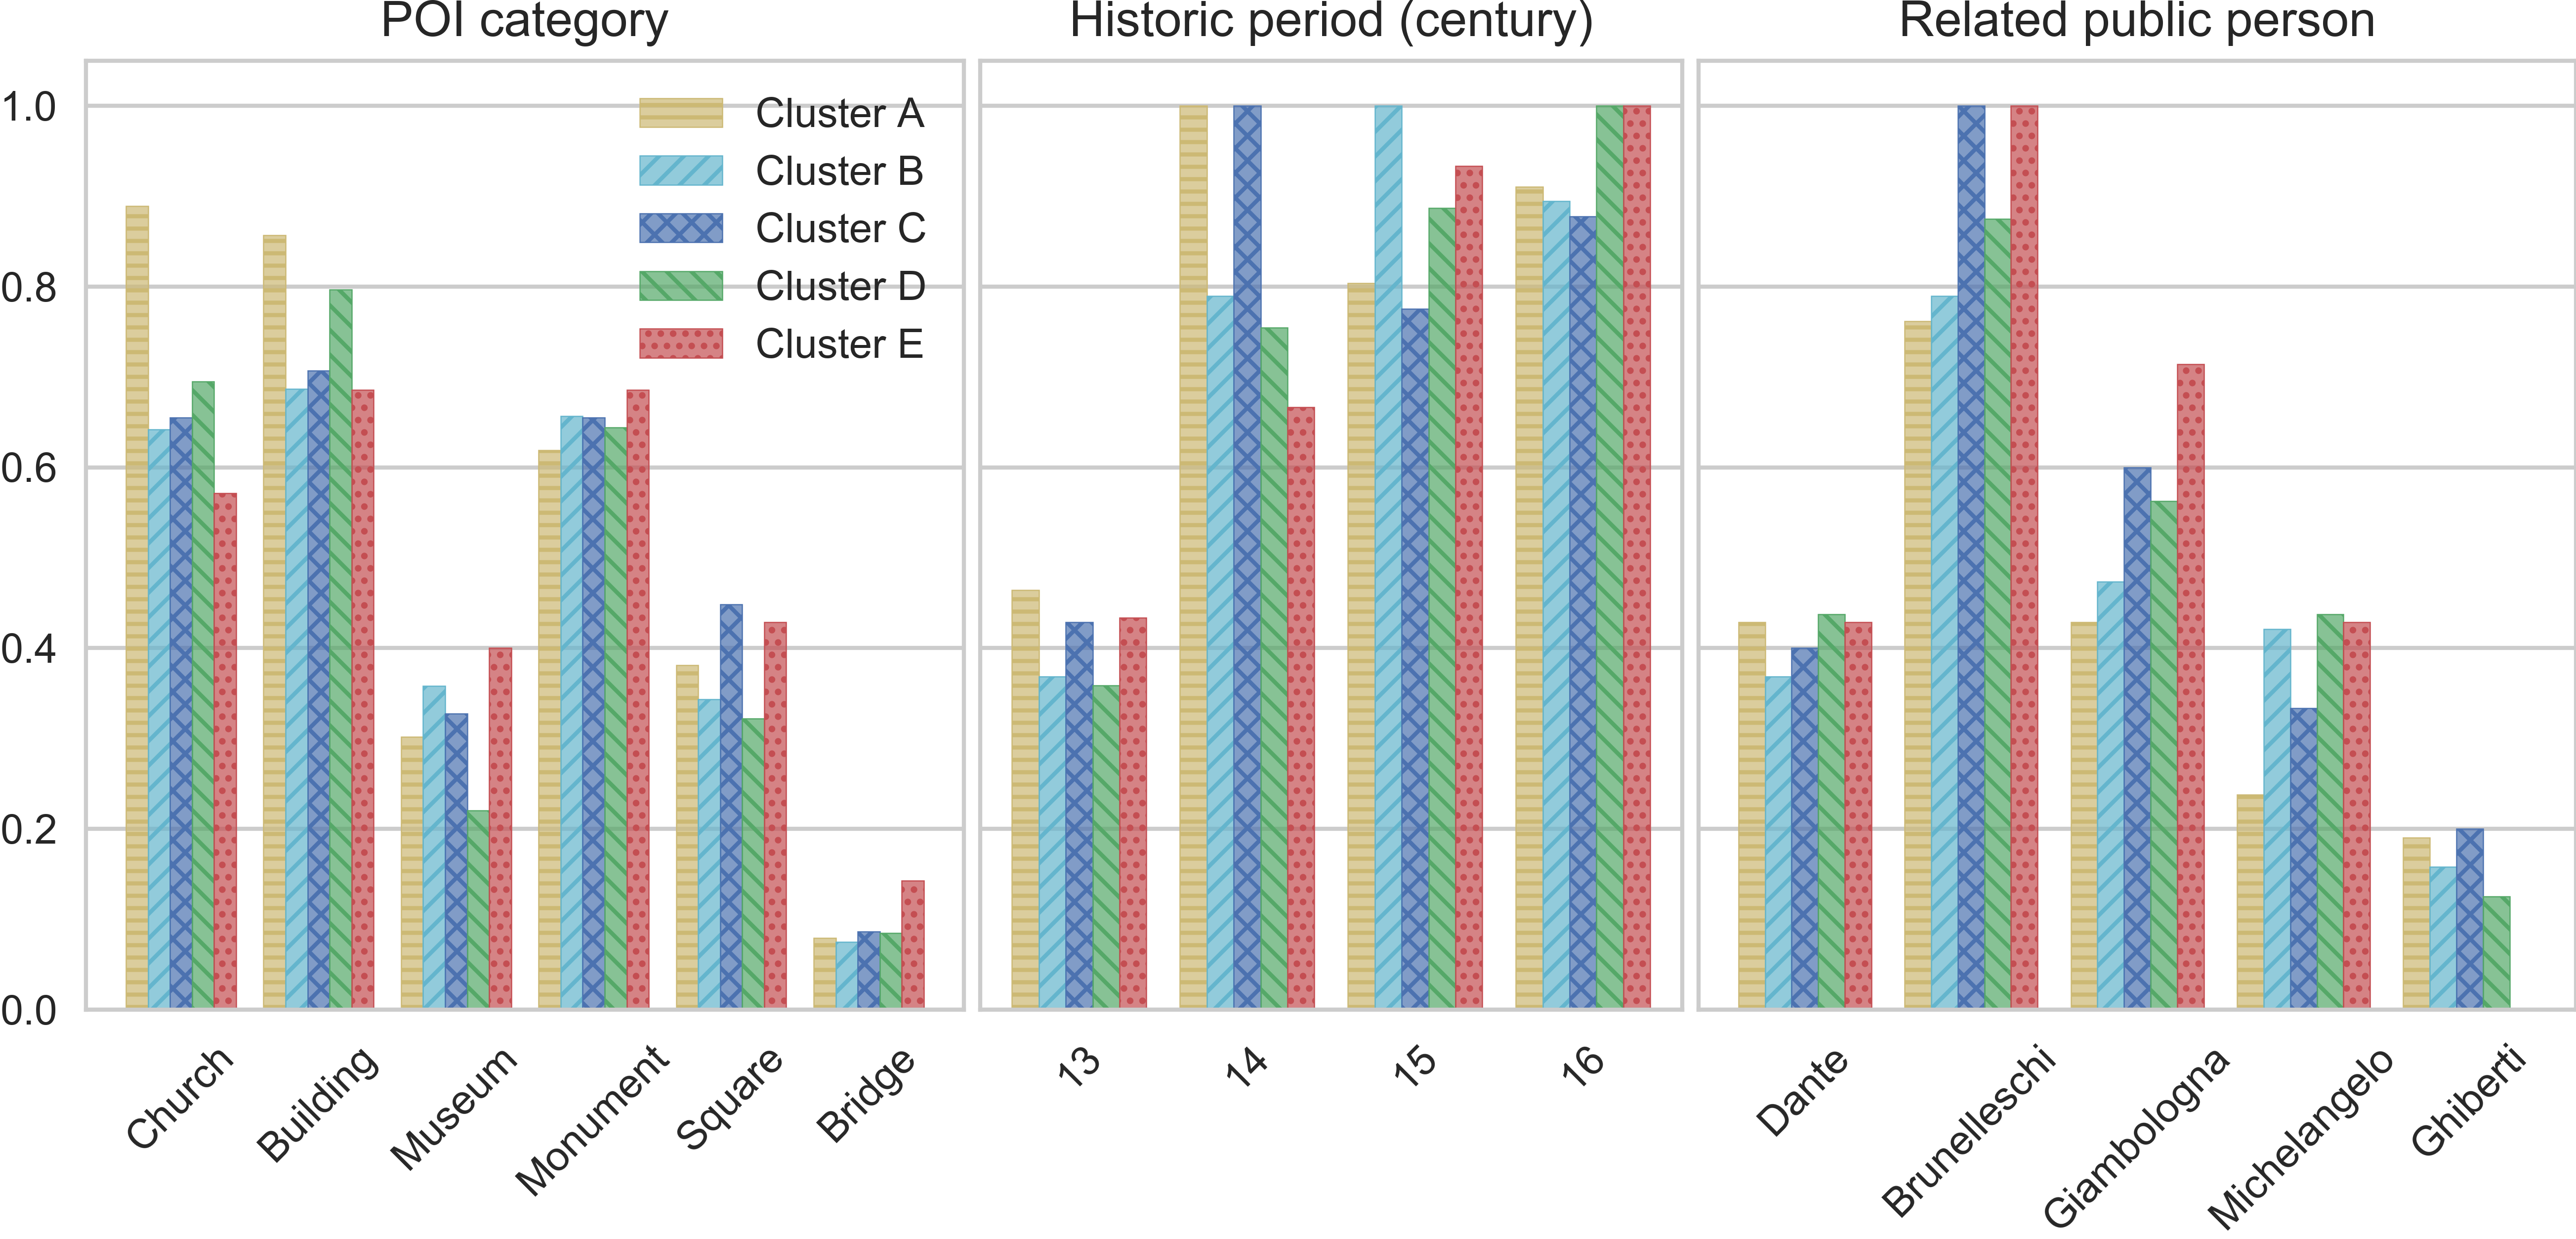
\includegraphics[width=1\linewidth]{cluster_comparison_poifeatures}
	\caption{Extract of POI features distribution per cluster.}
	\label{fig:cluster_poi}
\end{figure} 

Overall, we can see that the features variability in the clusters is not high. In fact, POIs are rather similar, i.e., they are mostly cultural POIs. It is reasonable to conjecture that if a more diverse assortment of POIs (e.g., leisure, restaurant, bar, etc.) were available then the clusters may have better discriminated alternative groups/types of tourists. Nevertheless, by looking at the specific POI descriptive features, one can notice interesting differences. For instance, POI categories like churches and buildings characterise mostly visits in clusters A and D, whereas to a lower extent trajectories in the other clusters (e.g., cluster E). Instead, cluster E is more representative of visits to bridges, squares and museums. Also POI historic period and POI related person features differentiate the clusters. For instance, cluster E is characterised by visits to POIs from the $15^{th}$ and $16^{th}$ centuries and artists from these times (i.e., Brunelleschi, Michelangelo and Giambologna).
Other relations between historic period and related person can be identified in $13^{th}$ century and Dante (e.g., clusters A and C) as well as $13^{th}$ century and Ghiberti (e.g., cluster A). Carrying out this analysis with a domain expert, an art historian, could reveal more similarities and differences between the clusters. 

In Figure \ref{fig:cluster_contex} we show the probabilities to observe certain context features in the clusters. For instance, by looking at the clusters C and E we can see that they mainly group  visits during cloudy days (left). Considering instead the temperature (centre), the clusters capture other nuances of the visits. For instance, cluster A represents visits in cold days, whereas cluster C groups visits in warmer days. Interestingly, focusing on the part of the day (right), there are clusters that represent visits performed at different times. For instance, mornings and afternoons in cluster A, afternoons and evenings in clusters B and over the whole day cluster D. 

By means of a $\chi^2$ test of independence, it has been found that the frequency of POI category, historic period, related person and weather depend on the cluster (all significant with $p<0.04$).

\begin{figure}
	\centering
	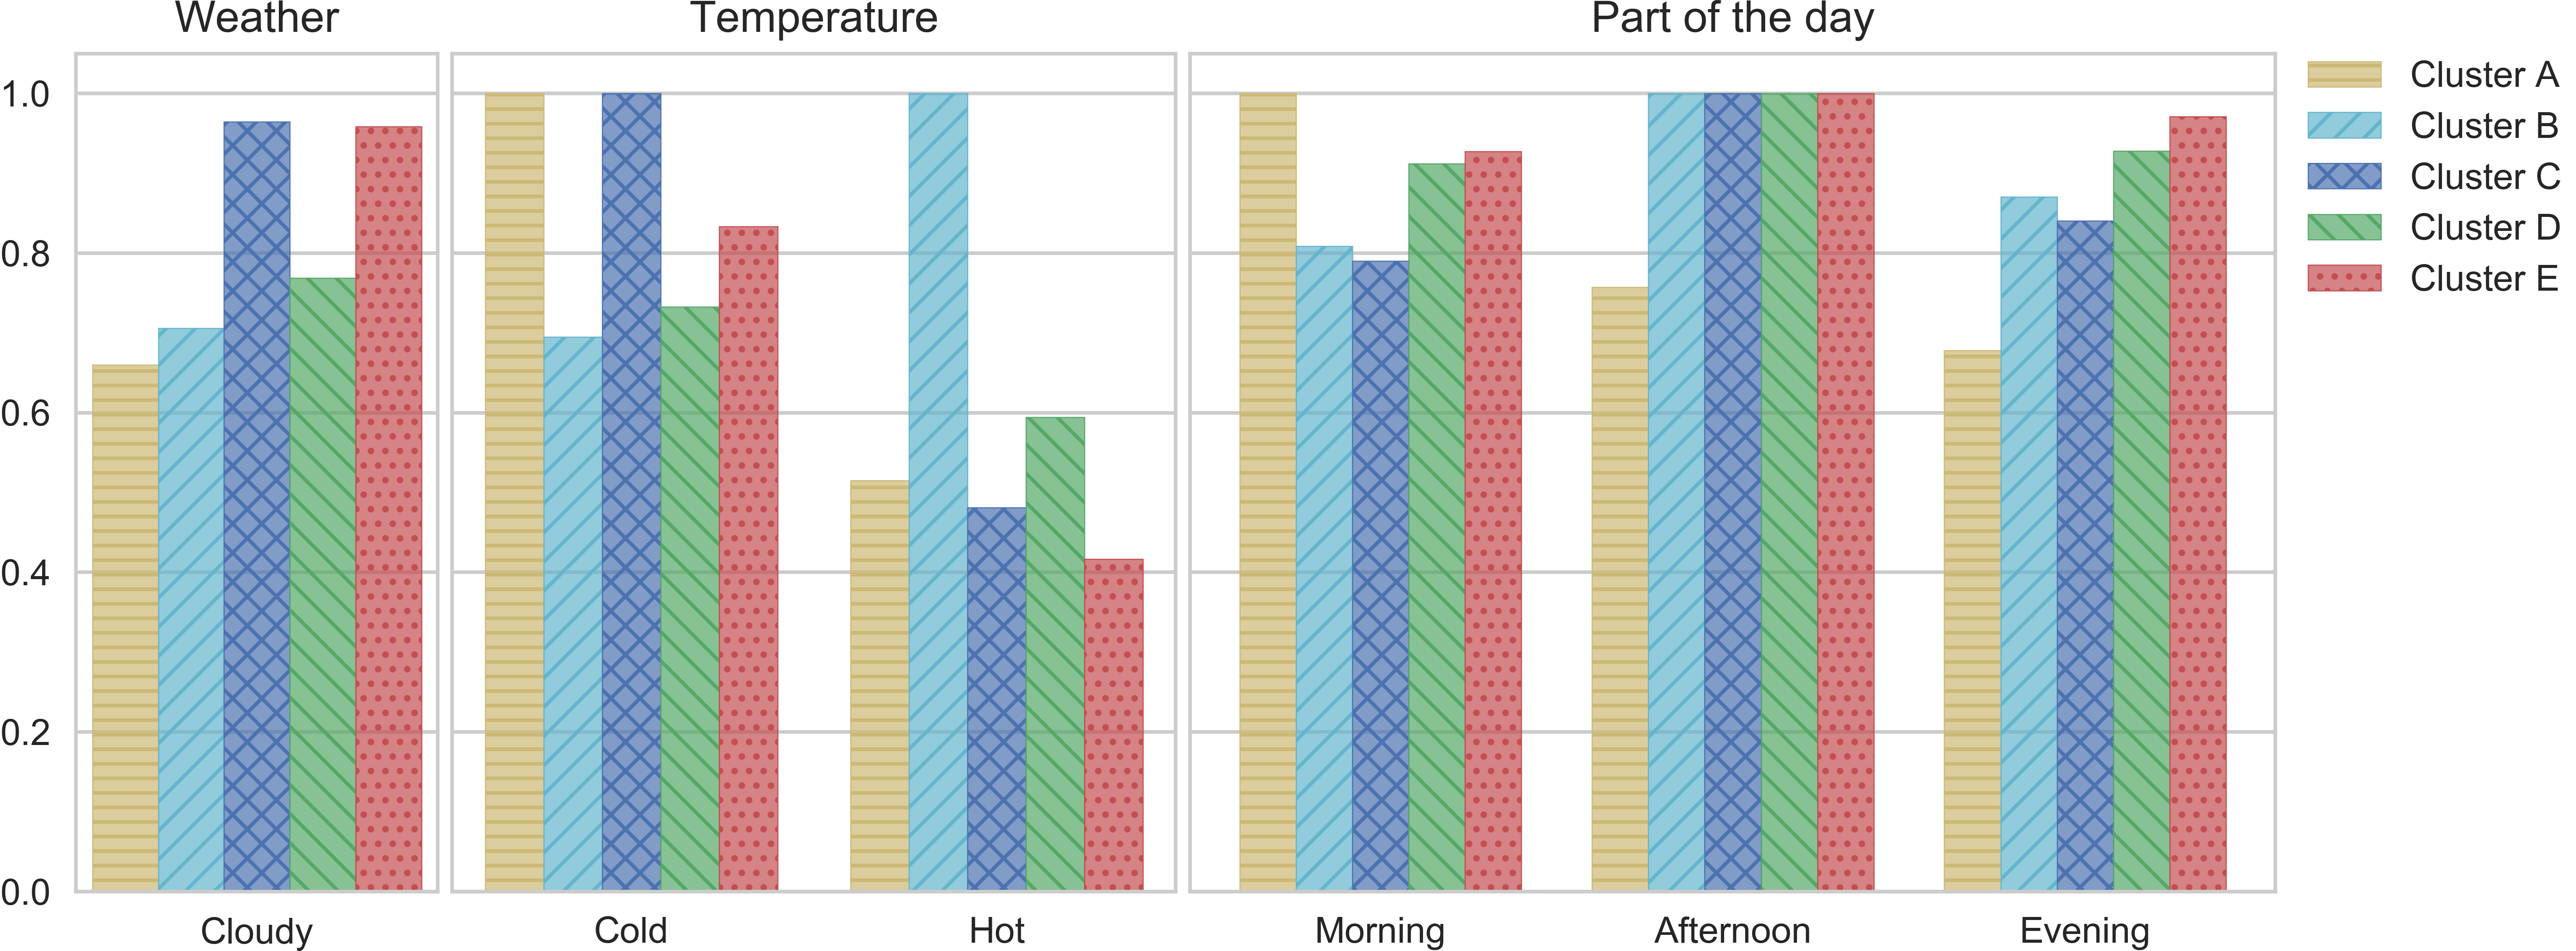
\includegraphics[width=1\linewidth]{cluster_comparison_contextfeatures}
	\caption{Extract of context features distribution per cluster.}
	\label{fig:cluster_contex}
\end{figure}

\subsection{MDP modelling}
%FR questa parte messa qui separata dal 4.3.1 non ha molto senso. Avrebbe piu' senso dire in 4.3.1 qualcosa di piu' sulla rappresentazione dello stato nelle nostre applicazioni e magari qui dare solo i dettagli. Ma forse questi dettagli si possono dare quando parli del data set delle traiettorie. Puoi descrivere il tuo MDP prima di parlare di clustering. 

We model each POI-visit trajectory in a cluster as the itinerary followed by a user, who is belonging to a group of like-minded users, that is taking decision as to optimize an (unknown) reward function common to all the users in the cluster. This problem is modelled as an MDP. 
%%FR sono un po' confuso. Il modello MDP lo hai mostrato nella sezione 4.3.1 Qui devi fare riferimento al modello generale e dire come i vari ingredienti si concretizzano per questa applicazione al turismo che usa questo particolare data set.

Let $P$ be the set of POIs visited by the users and let $\phi(s)$ 
%%FR e' la stessa phi di cui parlavi prima? Metti delle connessioni. phi e' la rappresentazione dello stato. E' lo stato un poi? Sembra che usi i due termini in maniera intercambiabile, ma devi fare distinzione tra i due, perche' non sono la stessa cosa. Il POI e' il punto di interesse, lo stato rappresenta la presenza del turista nel punto di interesse in un particolare contesto.
be the binary vector that represents for each POI the presence or absence of the following attributes: weather \textit{$f_w$}, where $w \in$ \textit{$\{$clear, foggy, partly cloudy, mostly cloudy, rainy, windy$\}$}; temperature \textit{$f_t$}, where $t \in $ \textit{$\{$freezing, cold, warm,hot$\}$}; daytime \textit{$f_d$}, where $d \in$ \textit{$\{$morning, afternoon, evening, night$\}$}; 
POI category \textit{$f_c$}, where $c \in$ \textit{$\{$church, \dots, palace$\}$}; historic period \textit{$f_h$}, where $h \in$  \textit{$\{3^{rd}$ century, \dots, $20^{th}$ century$\}$}; related person \textit{$f_r$}, where $r \in$ \textit{$\{$Brunellschi, \dots, Vasari$\}$}. 
In total there are 151 Boolean features ($F=151$), 137 representing the POI ($X=137$) and 14 representing the context ($C=14$). 

We define the state space as $S = P \times C $ where a state $s$ models the visit of a tourist at a specific POI in context.

In our problem a tourist can reach from a POI any other POI, therefore the set of actions is $A=P$. It is important to highlight that reaching a POI to visit next, i.e., performing an action, is a stochastic process: following action $a$ to reach a next POI may lead to the desired place with different context conditions, e.g., at Battistero can be rainy or foggy.

We denote with $\zeta_u$ a user $u$ trajectory, which is a temporally ordered list of states. For instance, $\zeta_{u_1} = (s_{10}, s_5, s_{15})$ represent a user $u_1$ trajectory starting from state $s_{10}$, moving to $s_5$ and ending to $s_{15}$.
%%FR queste cose le hai gia' dette.

The transition model $T$ is derived from the clustered trajectories.
%%FR queste cose le hai gia' dette.
Since we are interested in learning long term reward, i.e., optimizing for the whole visit, we set $\gamma=0.9$.


\subsection{Tourist behaviour}
In the second version of the thesis I will show the learnt behaviour models (per cluster) by showing why user's acted in a specific way. 
%%FR non e' molto chiaro cosa vuoi mostrare.